% siminos/spatiotemp/chapter/symm2d.tex
% $Author: predrag $ $Date: 2019-05-09 18:30:52 -0400 (Thu, 09 May 2019) $

The $d=2$ \catlatt\ has \textbf{p4m} symmetry:
square lattice, point group $D_4$, two rotation centres of order four (90${}^0$),
and reflections in four distinct directions (horizontal, vertical, and
diagonals). This corresponds to a straightforward grid of rows and columns of
equal squares with the four reflection axes.

The $d=2$ Lorentz gas has \textbf{p6m} symmetry: hexagonal lattice, point group
$D_6$. A pattern with this symmetry can be looked upon as a tessellation of the
plane with equal triangular tiles with D3 symmetry, or equivalently, a
tessellation of the plane with equal hexagonal tiles with D6 symmetry (with the
edges of the tiles not necessarily part of the pattern). Thus the simplest
examples are a triangular lattice with or without connecting lines, and a
hexagonal tiling with one color for outlining the hexagons and one for the
background.

There are five lattice types or Bravais lattices, corresponding to the five
possible wallpaper groups of the lattice itself. The wallpaper group of a
pattern with this lattice of translational symmetry cannot have more, but may
have less symmetry than the lattice itself.

The wallpaper groups \HREF{https://en.wikipedia.org/wiki/Wallpaper_group}
{wiki} has many online drawing tools.
                                                        \toCB

\subsection{$C_{4v}$ factorization}
\label{C-4v-inva}
% Predrag                               20sep2017
% extracted from appendSymm.tex {Discrete symmetries of dynamics}
% Predrag                               11apr2015

If an $N$-disk arrangement has $C_N$ symmetry, and the disk visitation
sequence is given by disk labels $\{ \epsilon_1 \epsilon_2 \epsilon_3 \dots\}$,
only the relative increments
$\rho_i = \epsilon_{i+1}-\epsilon_{i} \,\, {\rm mod\ } N$ matter.
Symmetries under reflections across axes increase the group to $C_{Nv}$ and
add relations between symbols: $\{\epsilon_i\}$ and $\{N - \epsilon_i\}$
differ only by a reflection. %\rf{tdisk,grass}.
As a consequence of this
reflection increments become decrements until the next reflection and
vice versa. Consider four equal disks placed on the vertices
of a square (\reffig{apeDscr:C4vSymm}). The symmetry group consists
of the identity $\bf e$, the two reflections $\sigma_x$, $\sigma_y$
across $x$, $y$ axes, the two diagonal reflections
$\sigma_{13}$, $\sigma_{24}$,
and the three rotations $C_4$, $C_2$ and $C_4^3$ by
angles $\pi/2$, $\pi$ and $3\pi/2$.
We start by exploiting the $C_4$ subgroup symmetry in order to
replace the absolute labels
$\epsilon_i \in \{ 1,2,3,4\}$ by relative increments $\rho_i \in \{ 1,2,3\}$.
By reflection across diagonals, an
increment by $3$ is equivalent to an increment by $1$ and a reflection;
this new symbol will be called $\underline{1}$.
Our convention will be to first perform
the increment and then to change the orientation due to the reflection.
As an example, consider the fundamental domain cycle
$112$. Taking the disk 1 $\rightarrow$
disk 2 segment as the starting segment, this symbol string
is mapped into the disk visitation sequence
$1_{+1} 2_{+1} 3_{+2}1 \dots= \overline{123}$, where the subscript
indicates the increments (or decrements) between neighboring symbols;
the period of the cycle $\overline{112}$
is thus 3 in both the fundamental domain and
the full space. Similarly, the cycle
$\overline{\underline{1}12}$ will be mapped into
$1_{+1} 2_{-1} 1_{-2} 3_{-1} 2_{+1} 3_{+2}1= \overline{121323}$
(note that the fundamental domain symbol $\underline{1}$
corresponds to a flip in orientation
after the second and fifth symbols);
%
%%%%%%%%%%%%%%%%%%%%%%%%%%%%%%%%%%%%%%%%%%%%%%%%%%%%%%%%%%%%%%%
% 20Jan2008: replaced f_4_disk_C4v_symm.eps
% by FigSrc/sune/c4v.eps from 1997-01-19, PC edit 2009-01-18
% old {fgC4v}
\SFIG{c4v}
{}{
Symmetries of four disks on a square.
A fundamental domain indicated by the shaded wedge.
}
{apeDscr:C4vSymm}
%%%%%%%%%%%%%%%%%%%%%%%%%%%%%%%%%%%%%%%%%%%%%%%%%%%%%%%%%%%%%%%
%
this time the period in the full space
is twice that of the fundamental domain. In particular, the
fundamental domain fixed points correspond to the following
4-disk cycles:
\vskip 12pt
\begin{center}
\begin{tabular}{lcr}
4-disk            &                    & reduced \\
$ {12} $ & $ \leftrightarrow $ & $ {\underline{1}} $ \\
$ {1234} $ & $ \leftrightarrow $ & $ {1} $ \\
$ {13} $ & $ \leftrightarrow $ & $ {2} $
\end{tabular}
\end{center}
\vskip 12pt
Conversions for all periodic orbits of reduced symbol period
less than 5 are listed in \reftab{t-symm-6}.

    \PublicPrivate{
    }{% switch \PublicPrivate{
    \PC{2009-01-18}{redrew FigSrc/sune/xfig/ .
    dynamics.fig is now renamed c4vRelative.fig,
    see \reffig{apeDscr:c4vRelative}. Try to find
    fig2.eps?
     }
%
%%%%%%%%%%%%%%%%%%%%%%%%%%%%%%%%%%%%%%%%%%%%%%%%%%%%%%%%%%%%%%%
% 18Jan2009: redrew FigSrc/sune/xfig/c4vRelative.fig
\FIG{
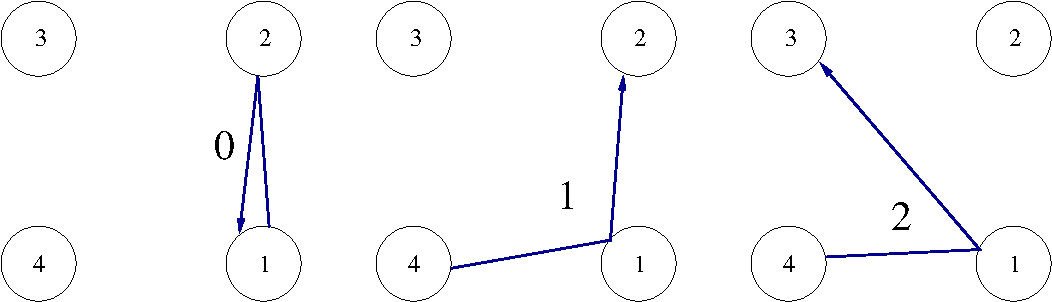
\includegraphics[width=0.66\textwidth]{c4vRelative}
}{}{
Reduced, fundamental domain symbolic dynamics for
four disks on a square.
}{apeDscr:c4vRelative}
%%%%%%%%%%%%%%%%%%%%%%%%%%%%%%%%%%%%%%%%%%%%%%%%%%%%%%%%%%%%%%%
%
\toSect{s-HamEqs}
    }% end \PublicPrivate{

%Table 6%%%%%%%%%%%%%%%%%%%%%%%%%%%%%%%%%%%%%%%%%%%%%%%%%%%%%%%
\begin{table}
\caption[]{\small
$C_{4v}$ correspondence between the ternary
fundamental
domain prime cycles $\tilde{p}$ and the full 4-disk \{1,2,3,4\}
labeled cycles ${p}$,
together with the $C_{4v}$ transformation that maps the end point of the
$\tilde{p}$ cycle into an irreducible segment of the $p$ cycle.
For typographical convenience, the symbol $\underline{1}$
of \refsect{C-4v-inva} has been replaced
by $0$, so that the ternary alphabet is $\{0,1,2\}$. The degeneracy
of the $p$ cycle is $m_p=8 \cl{\tilde{p}}/\cl{p}$.
Orbit $\overline{2}$ is the sole boundary orbit,
invariant both under a rotation by $\pi$
and a reflection across a diagonal. The two pairs of cycles
marked by $(a)$ and $(b)$ are related by time reversal, but cannot
be mapped into each other by $C_{4v}$ transformations.}
{\small
\begin{tabular}{lll}
$\tilde{p}$ & ${p}$  & ${\bf h}_{\tilde{p}}$ \\
\hline
0  &  1\,2  &  ${\sigma}_x$ \\
1  &  1\,2\,3\,4  &  $C_4$ \\
2  &  1\,3  &  $C_2$, ${\sigma}_{13}$ \\
%\hline
01  &  12\,14  &  ${\sigma}_{24}$ \\
02  &  12\,43  &  ${\sigma}_y$ \\
12  &  12\,41\,34\,23  &  $C_4^3$ \\
%\hline
001  &  121\,232\,343\,414  &  $C_4$ \\
002  &  121\,343  &  $C_2$ \\
011  &  121\,434  &  ${\sigma}_y$ \\
012  &  121\,323  &  ${\sigma}_{13}$ \\
021  &  124\,324  &  ${\sigma}_{13}$ \\
022  &  124\,213  &  ${\sigma}_x$ \\
112  &  123  &  $e$ \\
122  &  124\,231\,342\,413  &  $C_4$ \\
     &            & \\
     &            & \\
     &            & \\
     &            &
\end{tabular}%
~~~~~~%
\begin{tabular}{lll}
$\tilde{p}$ & ${p}$  & ${\bf h}_{\tilde{p}}$ \\
\hline
0001  &  1212\,1414  &  ${\sigma}_{24}$ \\
0002  &  1212\,4343  &  ${\sigma}_y$ \\
0011  &  1212\,3434  &  $C_2$ \\
0012  &  1212\,4141\,3434\,2323 & $C_4^3$~~~$\*$ \\
0021\ $(a)$ &  1213\,4142\,3431\,2324  &  $C_4^3$ \\
0022  &  1213  &  $e$ \\
0102\ $(a)$  &  1214\,2321\,3432\,4143 & $C_4$~~~$\*$ \\
0111  &  1214\,3234  &  ${\sigma}_{13}$ \\
0112\ $(b)$  &  1214\,2123  &  ${\sigma}_x$ \\
0121\ $(b)$  &  1213\,2124  &  ${\sigma}_x$ \\
0122  &  1213\,1413  &  ${\sigma}_{24}$ \\
0211  &  1243\,2134  &  ${\sigma}_x$ \\
0212  &  1243\,1423  &  ${\sigma}_{24}$ \\
0221  &  1242\,1424  &  ${\sigma}_{24}$ \\
0222  &  1242\,4313  &  ${\sigma}_y$ \\
1112  &  1234\,2341\,3412\,4123  &  $C_4$ \\
1122  &  1231\,3413  &  $C_2$ \\
1222  &  1242\,4131\,3424\,2313  &  $C_4^3$
\end{tabular}
} %end\small
\label{t-symm-6}
\end{table}


This symbolic dynamics is closely related
to the group-theoretic structure of the dynamics: the global
4-disk trajectory can be generated by mapping the fundamental domain
trajectories onto the
full 4-disk space by the accumulated product of the $C_{4v}$ group elements
$g_1=C$, $g_2=C^2$, $g_{\underline{1}}=\sigma_{diag} C= \sigma_{axis}$,
where $C$ is a rotation by $\pi/2$. In the $\overline{\underline{1}12}$
example worked out above, this yields
$g_{\underline{1}12} = g_{2} g_{1} g_{\underline{1}}
= C^2  C \sigma_{axis} = \sigma_{diag}$, listed in the last column of
\reftab{t-symm-6}.
Our convention is to multiply group elements in the reverse order with
respect to the symbol sequence.
We need these group elements for our next step,
the \dzeta\  factorizations.

%
%%%%%%%%%%%%%%%%%%%%%%%%%%%%%%%%%%%%%%%%%%%%%%%%%%%%%%%%%%%%%%%
\SFIG{f_4_disk_C2v_symm}
{}{
Symmetries of four disks on a rectangle.
A fundamental domain indicated by the shaded wedge.
}
{f_4_disk_C4v_symm}
%%%%%%%%%%%%%%%%%%%%%%%%%%%%%%%%%%%%%%%%%%%%%%%%%%%%%%%%%%%%%%%
%
The $C_{4v}$ group has four 1-dimensional representations, either symmetric
($A_1$) or antisymmetric ($A_2$) under both types of reflections, or symmetric
under one and antisymmetric under the other ($B_1$, $B_2$), and a
degenerate pair of
2-dimensional representations $E$. Substituting the $C_{4v}$ characters
\vskip .3cm
\begin{center}
\begin{tabular}{c|crrrr}
$C_{4v}$       & $A_1$& $A_2$& $B_1$& $B_2$& $E$ \\
\hline
$  e  $        &   1  &   1  &  1   &  1   &  2  \\
$C_2  $        &   1  &   1  &  1   &  1   & -2  \\
$C_4,C_4^3  $  &   1  &   1  & -1   & -1   &  0  \\
$\sigma_{axes}$&   1  &  -1  &  1   & -1   &  0  \\
$\sigma_{diag}$&   1  &  -1  & -1   &  1   &  0
\end{tabular}
\end{center}
\vskip .3cm
\noindent
into (\ref{zet-fac}) we obtain:
\vskip 12pt
\begin{tabular}{rlcccccc}

$h_{\tilde p}$ &  & &  $A_1$  &  $A_2$  &  $B_1$  &  $B_2$  &  $E$  \\
$e$:
& $(1-t_{\tilde p} )^8$  &=&$(1-t_{\tilde p})$ & $(1-t_{\tilde p})$ &
                        $(1-t_{\tilde p})$ &$(1-t_{\tilde p})$&$ (1-t_{\tilde
 p})^4 $ \\
$C_2$:
& $(1-t_{\tilde p}^2 )^4$ &=&  $(1-t_{\tilde p})$ & $(1-t_{\tilde p})$ &
                        $(1-t_{\tilde p})$ &$(1-t_{\tilde p})$&$ (1+t_{\tilde
 p})^4 $ \\
$C_4,C_4^3$:
& $(1-t_{\tilde p}^4 )^2$ &=&  $(1-t_{\tilde p})$ & $(1-t_{\tilde p})$ &
                        $(1+t_{\tilde p})$ &$(1+t_{\tilde p})$&$ (1+t_{\tilde
 p}^2)^2 $ \\
$\sigma_{axes}$:
& $(1-t_{\tilde p}^2 )^4$&=& $(1-t_{\tilde p})$ & $(1+t_{\tilde p})$ &
                        $(1-t_{\tilde p})$ &$(1+t_{\tilde p})$&$ (1-t_{\tilde
 p}^2)^2 $ \\
$\sigma_{diag}$:
& $(1-t_{\tilde p}^2 )^4$&=& $(1-t_{\tilde p})$ & $(1+t_{\tilde p})$ &
                        $(1+t_{\tilde p})$ &$(1-t_{\tilde p})$&$ (1-t_{\tilde
 p}^2)^2 $ \\
\end{tabular}
\vskip 12pt
\noindent
The possible irreducible segment
group elements ${\bf h}_{\tilde{p}}$ are listed in the first
column; $\sigma_{axes}$ denotes a reflection across either the x-axis or the
y-axis, and $\sigma_{diag}$ denotes a reflection across a diagonal
(see \reffig{apeDscr:C4vSymm}).

In addition, degenerate pairs of boundary orbits can
run along the symmetry lines in the full space, with the fundamental domain
group theory weights
${\bf h}_p=(C_2+\sigma_x)/2$ (axes) and
${\bf h}_p=(C_2+\sigma_{13})/2$ (diagonals) respectively:
\bea
  & & \quad A_1   \quad \quad  A_2  \quad \quad  B_1
      \quad \quad  B_2  \quad \quad  E  \continue
\mbox{axes:}\quad  (1-t_{\tilde{p}}^2)^2 & = &
(1-t_{\tilde{p}})(1-0 t_{\tilde{p}})
(1-t_{\tilde{p}})(1-0 t_{\tilde{p}}) (1+t_{\tilde{p}})^2
\continue
\mbox{diagonals:}\quad  (1-t_{\tilde{p}}^2)^2 & = &
(1-t_{\tilde{p}})(1-0 t_{\tilde{p}})
(1-0 t_{\tilde{p}})(1- t_{\tilde{p}}) (1+t_{\tilde{p}})^2
\label{bounda4}
\eea
(we have assumed that $t_{\tilde{p}}$ does not change sign under
reflections across symmetry axes).
For the 4-disk arrangement considered here
only the diagonal orbits $\overline{13}$,
$\overline{24}$ occur; they correspond to the
$\overline{2}$ fixed point in the fundamental domain.

The $A_1$ subspace in $C_{4v}$ cycle expansion
is given by
\bea
1/\zeta_{A_1} & = & (1-t_{0})(1-t_{1})(1-t_{2})
     (1-t_{01})(1-t_{02})(1-t_{12}) \ceq
     (1-t_{001})(1-t_{002})(1-t_{011})(1-t_{012})
     (1-t_{021})(1-t_{022})(1-t_{112}) \ceq (1-t_{122})
     (1-t_{0001})(1-t_{0002})(1-t_{0011})(1-t_{0012})(1-t_{0021})
            \dots \continue
 &= &  1 - t_0 - t_1 - t_2
 - (t_{01}- t_0 t_1) - (t_{02} - t_0 t_2) - (t_{12} - t_1 t_2) \ceq
- (t_{001} - t_0 t_{01}) - (t_{002} - t_0 t_{02}) - (t_{011} - t_1 t_{01}) \ceq
- (t_{022} - t_2 t_{02}) - (t_{112} - t_1 t_{12}) - (t_{122} - t_2 t_{12}) \ceq
- (t_{012} + t_{021} + t_0 t_1 t_2 - t_0 t_{12} - t_1 t_{02} - t_2 t_{01})
\dots
\label{zc4vA1}
\eea
(for typographical convenience, $\underline{1}$ is replaced by $0$ in
the remainder of this section).
For 1-dimensional representations, the characters can be read off
the symbol strings:
$
\chi_{A_2}({\bf h_{\tilde{p}} }) = (-1)^{n_0}
$,
$
\chi_{B_1}({\bf h_{\tilde{p}} }) = (-1)^{n_1 }
$,
$
\chi_{B_2}({\bf h_{\tilde{p}} }) = (-1)^{n_0+n_1 }
$,
where $n_{0}$ and $n_1$ are the number of times symbols ${0}$, $1$ appear in
the $\tilde{p}$ symbol string.
For $B_2$ all $t_p$ with an odd total number of $0$'s and $1$'s change sign:
\bea
1/\zeta_{B_2} & = & (1+t_{0})(1+t_{1})(1-t_{2})
     (1-t_{01})(1+t_{02})(1+t_{12}) \ceq
     (1+t_{001})(1-t_{002})(1+t_{011})(1-t_{012})
     (1-t_{021})(1+t_{022})(1-t_{112}) \ceq (1+t_{122})
     (1-t_{0001})(1+t_{0002})(1-t_{0011})(1+t_{0012})(1+t_{0021})
            \dots \continue
 &= &  1 + t_0 + t_1 - t_2
 - (t_{01}- t_0 t_1) + (t_{02} - t_0 t_2) + (t_{12} - t_1 t_2) \ceq
+ (t_{001} - t_0 t_{01}) - (t_{002} - t_0 t_{02}) + (t_{011} - t_1 t_{01}) \ceq
+ (t_{022} - t_2 t_{02}) - (t_{112} - t_1 t_{12}) + (t_{122} - t_2 t_{12}) \ceq
- (t_{012} + t_{021} + t_0 t_1 t_2 - t_0 t_{12} - t_1 t_{02} - t_2 t_{01})
\dots
\label{zc4vB2}
\eea
The form of the remaining cycle expansions depends
crucially on the special role played by the boundary
orbits: by (\ref{bounda4}) the orbit $t_2$ does not contribute
to $A_2$ and $B_1$,
\bea
1/\zeta_{A_2} & = & (1+t_{0})(1-t_{1})
     (1+t_{01})(1+t_{02})(1-t_{12}) \ceq
     (1-t_{001})(1-t_{002})(1+t_{011})(1+t_{012})
     (1+t_{021})(1+t_{022})(1-t_{112}) \ceq (1-t_{122})
     (1+t_{0001})(1+t_{0002})(1-t_{0011})(1-t_{0012})(1-t_{0021})
            \dots \continue
 &= &  1 + t_0 - t_1
 + (t_{01} - t_0 t_1) + t_{02} - t_{12} \ceq
 - (t_{001} - t_0 t_{01}) - (t_{002} - t_0 t_{02}) + (t_{011} - t_1 t_{01}) \ceq
 + t_{022} - t_{122} - (t_{112} - t_1 t_{12})
 + (t_{012} + t_{021} - t_0 t_{12} - t_1 t_{02})
\dots
\label{z4vA2}
\eea
and
\bea
1/\zeta_{B_1} & = & (1-t_{0})(1+t_{1})
     (1+t_{01})(1-t_{02})(1+t_{12}) \ceq
     (1+t_{001})(1-t_{002})(1-t_{011})(1+t_{012})
     (1+t_{021})(1-t_{022})(1-t_{112}) \ceq (1+t_{122})
     (1+t_{0001})(1-t_{0002})(1-t_{0011})(1+t_{0012})(1+t_{0021})
            \dots \continue
 &= &  1 - t_0 + t_1
 + (t_{01} - t_0 t_1) - t_{02} + t_{12} \ceq
 + (t_{001} - t_0 t_{01}) - (t_{002} - t_0 t_{02}) - (t_{011} - t_1 t_{01}) \ceq
 - t_{022} + t_{122} - (t_{112} - t_1 t_{12})
 + (t_{012} + t_{021} - t_0 t_{12} - t_1 t_{02})
\dots
\label{z4vB1}
\eea
In the above we have  assumed that $t_2$ does not change sign under $C_{4v}$
reflections.
For the mixed-symmetry subspace $E$ the curvature expansion is given by
\bea
1/\zeta_E &=&  1 + t_2  + ( -{{t_{0}}^2} + {{t_{1}}^2} )  +
   ( 2 t_{002} - t_2 {{t_{0}}^2} - 2 t_{112} + t_2 {{t_{1}}^2} )
  \ceq
   + ( 2 t_{0011} - 2 t_{0022} + 2 t_2 t_{002} - {{t_{01}}^2} -
      {{t_{02}}^2} + 2 t_{1122} - 2 t_2 t_{112}
  \ceq
 + {{t_{12}}^2} -  {{t_{0}}^2} {{t_{1}}^2} )
   +  ( 2 t_{00002} - 2 t_{00112} + 2 t_2 t_{0011} - 2 t_{00121}
      -  2 t_{00211}
  \ceq
 + 2 t_{00222} - 2 t_2 t_{0022} + 2 t_{01012}
 + 2 t_{01021} - 2 t_{01102}
 - t_2 {{t_{01}}^2} + 2 t_{02022}
            \ceq
   -    t_2 {{t_{02}}^2} + 2 t_{11112} - 2 t_{11222} + 2 t_2 t_{1122} -
      2 t_{12122} + t_2 {{t_{12}}^2}
 - t_2 {{t_{0}}^2} {{t_{1}}^2}
            \ceq
+  2 t_{002} ( -{{t_{0}}^2} + {{t_{1}}^2} )  -
      2 t_{112} ( -{{t_{0}}^2} + {{t_{1}}^2} )  )
\eea

A quick test of the
$\zeta= \zeta_{A_1} \zeta_{A_2} \zeta_{B_1} \zeta_{B_2} \zeta_E^2 $
factorization is afforded by the topological polynomial; substituting
$t_p = z^{\cl{p}}$ into the expansion yields
\[
1/\zeta_{A_1} = 1- 3 z \,\, , \quad
1/\zeta_{A_2}  = 1/\zeta_{B_1}  = 1 \,\, , \quad
1/\zeta_{B_2} = 1/\zeta_{E} = 1 +  z \,\, ,
\]\noindent
in agreement with (\ref{4disk-top}).
\exerbox{e_4-disk_zeta}



\subsection{$C_{2v}$ factorization}
\label{c2vinv}
% Predrag                               20sep2017
% extracted from appendSymm.tex {Discrete symmetries of dynamics}

An arrangement of four identical disks on the vertices of a rectangle has
$C_{2v}$ symmetry (\reffig{f_4_disk_C4v_symm}\,(b)). $C_{2v}$ consists of
$\{ {e}, {\sigma}_x, {\sigma}_y, {C}_2\}$, \ie,  the reflections
across the symmetry axes and a rotation by $\pi$.

This system affords a rather easy visualization of the  conversion of a 4-disk
dynamics into a fundamental domain symbolic dynamics. An orbit leaving the
fundamental domain through one of the axis may be folded back by a
reflection on that axis; with these symmetry operations
$g_0 = \sigma_x$ and $g_1 = \sigma_y$ we associate labels $1$ and $0$,
respectively. Orbits going to the diagonally opposed disk cross the
boundaries of the fundamental domain twice; the product of these
two reflections is just $C_2=\sigma_x \sigma_y$, to which we assign
the label $2$. For example, a ternary string $0\,0\,1\,0\,2\,0\,1\dots$
is converted into 12143123$\dots$, and the associated group-theory weight is
given by $\dots g_1 g_0 g_2 g_0 g_1 g_0 g_0 $.

Short ternary cycles and the corresponding 4-disk cycles
are listed in \reftab{t-symm-7}.
Note that already at length three there is a pair of
cycles (012~=~143 and 021~=~142) related by time
reversal, but {\em not} by any $C_{2v}$ symmetries.

%Table 7.
\begin{table}
\caption[]{\small
$C_{2v}$ correspondence between the ternary $\{0,1,2\}$
fundamental domain prime cycles $\tilde{p}$ and the full 4-disk \{1,2,3,4\}
cycles ${p}$, together with the $C_{2v}$ transformation that maps the end
point of the $\tilde{p}$ cycle into an irreducible segment of the $p$ cycle.
The degeneracy of the $p$ cycle is $m_p=4 \cl{\tilde{p}}/\cl{p}$. Note that the
$ 012$ and $ 021 $ cycles are related by time reversal,
but cannot be mapped into each other by $C_{2v}$ transformations. The full
space orbit listed here is generated from the symmetry reduced code by the
rules given in \refsect{c2vinv}, starting from disk 1.
}
{\small
\begin{tabular}{lll}
$\tilde{p}$ & $p$       &       ${ \bf g}$ \\ \hline
0       &       1\,4      &       ${ \sigma}_y$ \\
1       &       1\,2      &       ${ \sigma}_x$ \\
2       &       1\,3      &       ${ C}_2$ \\
%\hline
01      &       14\,32    &       ${ C}_2$ \\
02      &       14\,23    &       ${ \sigma}_x$ \\
12      &       12\,43    &       ${ \sigma}_y$ \\
%\hline
001     &       141\,232  &       ${ \sigma}_x$ \\
002     &       141\,323  &       ${ C}_2$ \\
011     &       143\,412  &       ${ \sigma}_y$ \\
012     &       143     &       ${ e}$ \\
021     &       142     &       ${ e}$ \\
022     &       142\,413  &       ${ \sigma}_y$ \\
112     &       121\,343  &       ${ C}_2$ \\
122     &       124\,213  &       ${ \sigma}_x$ \\
        &                 & \\
        &                 & \\
        &                 & \\
        &                 &
\end{tabular}%
~~~~~~%
\begin{tabular}{lll}
$\tilde{p}$ & $p$       &       ${ \bf g}$ \\ \hline
0001    &  1414\,3232 & ${C}_2$ \\
0002    &  1414\,2323 & ${\sigma}_x$ \\
0011    &       1412              & ${ e}$ \\
0012    &       1412\,4143        & ${ \sigma}_y$ \\
0021    &       1413\,4142        & ${ \sigma}_y$ \\
0022    &       1413              & ${ e}$ \\
0102    &       1432\,4123        & ${ \sigma}_y$ \\
0111    &       1434\,3212        &       ${ C}_2$ \\
0112    &       1434\,2343        &       ${ \sigma}_x$ \\
0121    &       1431\,2342        &       ${ \sigma}_x$ \\
0122    &       1431\,3213        &       ${ C}_2$ \\
0211    &       1421\,2312        &       ${ \sigma}_x$ \\
0212    &       1421\,3243        &       ${ C}_2$ \\
0221    &       1424\,3242        &       ${ C}_2$ \\
0222    &       1424\,2313        &       ${ \sigma}_x$ \\
1112    &       1212\,4343        &       ${ \sigma}_y$ \\
1122    &       1213    &       ${ e}$ \\
1222    &       1242\,4313        &       ${ \sigma}_y$
\end{tabular}
} %end\small
\label{t-symm-7}
\end{table}


The above is the complete description of the symbolic dynamics for 4
sufficiently separated equal
disks placed at corners of a rectangle. However, if
the fundamental domain requires further partitioning, the ternary description is
insufficient. For example, in the stadium billiard fundamental domain one has
to distinguish between bounces off the straight and the curved sections of the
billiard wall; in that case five symbols suffice for
constructing the covering symbolic dynamics.
\index{stadium billiard}
\index{billiard!stadium}
\PC{}{include paper with Kai?}

The group $C_{2v}$ has four 1-dimensional
representations, distinguished by their behavior under axis reflections.
The $A_1$ representation is symmetric with respect to both reflections;
the $A_2$ representation is antisymmetric with respect to both.
The $B_1$ and $B_2$ representations are symmetric under one
and antisymmetric under the other reflection. The character table is
\vskip .3cm
\begin{center}
\begin{tabular}{c|crrr}
$C_{2v}$    & $A_1$& $A_2$& $B_1$ & $B_2$\\
\hline
$ e   $       & $1$  & $ 1$  & $ 1$  & $ 1$  \\
$ C_2$        & $1$  & $ 1$  & $-1$  & $-1$  \\
$ \sigma_x$   & $1$  & $-1$  & $ 1$  & $-1$  \\
$ \sigma_{y} $& $1$  & $-1$  & $-1$  & $ 1$
\end{tabular}
\end{center}
\vskip .3cm

Substituted into the factorized determinant (\ref{factzet}),
the contributions of periodic orbits split as follows
\vskip 12pt
\begin{tabular}{rlccccc}

$g_{\tilde p}$
&  & &  $A_1$  &  $A_2$  &  $B_1$  &  $B_2$  \\
$e$:
& $(1-t_{\tilde p} )^4 $ &=&  $(1-t_{\tilde p})$ & $(1-t_{\tilde p})$ &
                        $(1-t_{\tilde p})$ &$(1-t_{\tilde p})$ \\
$C_2$:
& $(1-t_{\tilde p}^2 )^2$ &=&  $(1-t_{\tilde p})$ & $(1-t_{\tilde p})$ &
                        $(1-t_{\tilde p})$ &$(1-t_{\tilde p})$  \\
$\sigma_x$:
& $(1-t_{\tilde p}^2 )^2$&=& $(1-t_{\tilde p})$ & $(1+t_{\tilde p})$ &
                        $(1-t_{\tilde p})$ &$(1+t_{\tilde p})$ \\
$\sigma_{y}$:
& $(1-t_{\tilde p}^2 )^2$&=& $(1-t_{\tilde p})$ & $(1+t_{\tilde p})$ &
                        $(1+t_{\tilde p})$ &$(1-t_{\tilde p})$ \\
\end{tabular}
\vskip 12pt
\noindent
Cycle expansions follow by substituting cycles and their group
theory factors from \reftab{t-symm-7}.
For $A_1$ all characters are $+1$, and the corresponding cycle expansion is
given in (\ref{zc4vA1}).
Similarly, the totally antisymmetric subspace factorization $A_2$ is given by
(\ref{zc4vB2}),
the $B_2$ factorization of $C_{4v}$.
For $B_1$ all $t_p$ with an odd total number of $0$'s and $2$'s change sign:
\bea
1/\zeta_{B_1} & = & (1+t_{0})(1-t_{1})(1+t_{2})
     (1+t_{01})(1-t_{02})(1+t_{12}) \ceq
     (1-t_{001})(1+t_{002})(1+t_{011})(1-t_{012})
     (1-t_{021})(1+t_{022})(1+t_{112}) \ceq
     (1-t_{122})
     (1+t_{0001})(1-t_{0002})(1-t_{0011})(1+t_{0012})(1+t_{0021})
            \dots \continue
 &= &  1 + t_0 - t_1 + t_2
 + (t_{01}- t_0 t_1) - (t_{02} - t_0 t_2) + (t_{12} - t_1 t_2) \ceq
- (t_{001} - t_0 t_{01}) + (t_{002} - t_0 t_{02}) + (t_{011} - t_1 t_{01}) \ceq
+ (t_{022} - t_2 t_{02}) + (t_{112} - t_1 t_{12}) - (t_{122} - t_2 t_{12}) \ceq
- (t_{012} + t_{021} + t_0 t_1 t_2 - t_0 t_{12} - t_1 t_{02} - t_2 t_{01})
\dots
\label{zc2vB1}
\eea
For $B_2$ all $t_p$ with an odd total number of $1$'s and $2$'s change sign:
\bea
1/\zeta_{B_2} & = & (1-t_{0})(1+t_{1})(1+t_{2})
     (1+t_{01})(1+t_{02})(1-t_{12}) \ceq
     (1+t_{001})(1+t_{002})(1-t_{011})(1-t_{012})
     (1-t_{021})(1-t_{022})(1+t_{112}) \ceq
     (1+t_{122})
     (1+t_{0001})(1+t_{0002})(1-t_{0011})(1-t_{0012})(1-t_{0021})
            \dots \continue
 &= &  1 - t_0 + t_1 + t_2
+ (t_{01}- t_0 t_1) + (t_{02} - t_0 t_2) - (t_{12} - t_1 t_2) \ceq
+ (t_{001} - t_0 t_{01}) + (t_{002} - t_0 t_{02}) - (t_{011} - t_1 t_{01}) \ceq
- (t_{022} - t_2 t_{02}) + (t_{112} - t_1 t_{12}) + (t_{122} - t_2 t_{12}) \ceq
- (t_{012} + t_{021} + t_0 t_1 t_2 - t_0 t_{12} - t_1 t_{02} - t_2 t_{01})
\dots
\label{zc2vB2}
\eea
Note that all of the above cycle expansions group long orbits together
with their pseudo-orbit shadows,
so that the shadowing arguments for convergence still apply.

The topological polynomial factorizes as
\[
\frac{1}{\zeta_{A_1}} = 1-3z \quad,\quad
\frac{1}{\zeta_{A_2}} =
\frac{1}{\zeta_{B_1}} =
\frac{1}{\zeta_{B_2}} = 1 + z,
\]\noindent
consistent with the 4-disk factorization (\ref{4disk-top}).
\PC{}{add here Freddy p. 26; PER sect. 6.4.}

\subsection{Symmetries of the \topp}
% Predrag                               20sep2017
% extracted from appendSymm.tex {Discrete symmetries of dynamics}
\label{c-symbol-plane}

Depending on the type of dynamical system, the \topp\ might have
a variety of symmetries.
Under the time reversal
\[
   \biinf{\Ssym{-2}\Ssym{-1}\Ssym{0}}{\Ssym{1}\Ssym{2} \Ssym{3}}
\to
   \biinf{\Ssym{3}\Ssym{2}\Ssym{1}}{\Ssym{0}\Ssym{-1} \Ssym{-2}}
\]
the points in the  \topp\ for an \opres\ map are
symmetric across the diagonal $\gamma=\delta$, and
for the \orev\ case they are symmetric
with respect to the $\gamma=1-\delta$ diagonal.
Consequently the  periodic orbits appear either in dual pairs
$p=\Ssym{1} \Ssym{2} \Ssym{3} \ldots \Ssym{n}$,
$\overline{p}=\Ssym{n} \Ssym{n-1} \Ssym{n-2} \ldots \Ssym{1}$,
or are self-dual under time reversal,
$S_{p} = S_{\overline{p}}$.
% $\Ssym1 \Ssym2 \Ssym3 \ldots \Ssymn = \Ssymn \Ssym{n-1} \Ssym{n-2} \ldots \Ssym1$.
For the \opres\ case
a self-dual cycle of odd period has at least one point on the
symmetry diagonal. In particular, all fixed points lie on the symmetry
diagonal. Determination of such symmetry lines can be of considerable
practical utility, as it reduces some of the periodic orbit
searches to 1-dimensional searches.
